\section{Environment}
\label{sec:environment}

\subsection{SEAM4US}
\label{subsec:seam4us}

% TODO rephrase
Underground transportation systems have significant impacts on energy consumption at a regional scale. While the transportation systems, i.e. has high betrachtung hinsichtlich enery efficence, the subsystems of metro stations and surroundings, such as ventilation, vertical transportation and lightning are ?rarely? unexplored. Although a relatively small percentage of energy can be saved with an efficient management of these subsystems, a large energy saving in absolute terms can be obtained.
To research in the area of energy efficient surroundings the EU funded the "Sustainable Energy mAnageMent for Underground Stations"~(SEAM4US) project in Seventh Framework Programme.
"The objective of SEAM4US is to develop advanced technologies for optimal and scalable control of metro stations that will produce a 5\% saving in non-traction electricity consumption in one year, which is equivalent to the electricity consumed in more than 700 households. The project’s main outcomes will be the creation of systems for optimized integrated energy management, and the development of a decision support system to drive mid-term investments." TODO reference
SEAM4US will integrate additional energy metering and sensor-actuator networks with the existing systems (e.g. surveillance, passenger information and train scheduling)  to acquire grounded user, environmental and scheduling data. The data set will update and enable a set of adaptive energy consumption and environmental models to proactively and optimally control the metro stations.
The SEAM4US consortium consists of nine partners. A large metro network operator, TMB; a major player in energy-efficient system management sector, COFELY; building and environmental physics and construction experts UNIVPM and UPC, respectively; R+D experts in middleware, FhG FIT and VTT; R+D experts in user and agent-based scheduling modeling, ALMENDE and UNIKASSEL; system integrator, CNET. [TODO quelle angeben ggf. [www.seam4us.eu]


\subsection{Underground Station Passeig de Gr\`{a}cia}
\label{subsec:station}

The implementation of the developed advanced technologies is done in one of the stations of the partner TMB in Barcelona.
This section describes the "station" in detail. First the word "station" in the area of metro networks needs to be defined.

A metro network is composed by one or more metro lines. Each line has a fixed railway with a given number of stops to allow people to get on or off the trains by means of a platform: each of these stops is called "line station". A "metro station" is the concept that represents the point in space through which a passenger gets underground and into a line station. Metro station and line station can be the same physical entity, but it is possible that there are some "metro stations" that receive two or more "metro lines" in different platforms, and have therefore, two or more "line stations" within.

The data, used in this work, are gathered in line station in Passeig de Gr\`{a}cia - Line~3~(PdG-L3) in Barcelona. Passeig de Gr\`{a}cia~(PdG) is a station in the metro network of "Transports Metropolitans de Barcelona"~(TMB) and lies in a very iconic and touristic part of Barcelona. Some of the most popular buildings designed by Antoni Gaudi are in the proximity (Casa Batll\`{o}, Casa Mil\`{a}), as well as the city's most renown and exclusive boutiques.
The metro station is a historic icon of the Barcelona metro network. First opened in December of 1924, as a (line) station for Line~3, nowadays PdG holds three different line stations: L2, L3, and L4. The stations were built in three different periods and using different construction technologies in each of the premises (contemporary to the building periods). All line stations station has been refurbished a few times since 1924 and new equipment has been added recently.

Depending on the weekday PdG is open 19~hours, 21~hours or 24~hours. Between Monday and Thursday PdG service starts at 5:00 and ends at 24:00 (19~hours). Friday service starts at 5:00 and ends at 2:00 (21~hours). On Saturday service starts at 5:00 to but remain the entire night until midnight on Sunday.

Passeig~de~Gr\`{a}cia - Line~3~(PdG-L3) turns out to be representative for many station within TMBs metro network~\cite{TMB}. Moreover PdG-L3 is a crowded station which have low-rate usage hours as well. This provides a wide range of data which allows to test with very busy peak hours as well as with off-peaks. Figure~\ref{fig:PdG-L3_platforms} depicts the platforms of PdG-L3.

\begin{figure}[htb]
  \centering
  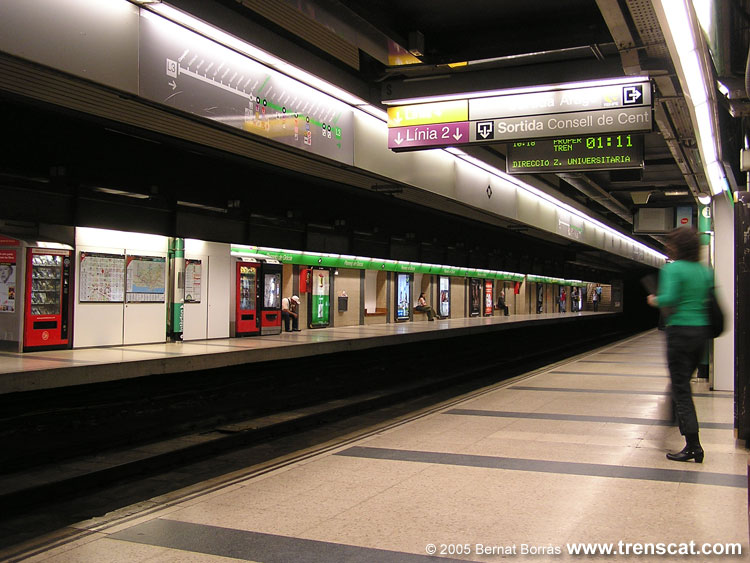
\includegraphics[width=\linewidth]{Figures/PdG-L3_platforms.jpg} 
  \caption{PdG-L3 Plattforms. \cite{TMB}}
  \label{fig:PdG-L3_platforms}
\end{figure}

The line station PdG-L3 consists of several public spaces: halls, transit areas, accesses to the platforms, and platforms. Furthermore there are private spaces such as technical rooms or staff dependencies. The private spaces are not part of the investigation in this work. Figure~\ref{fig:PdG-L3_schematic} depicts the line station schematic where the accesses to platforms are highlighted in red.

\begin{figure}[htb]
  \centering
  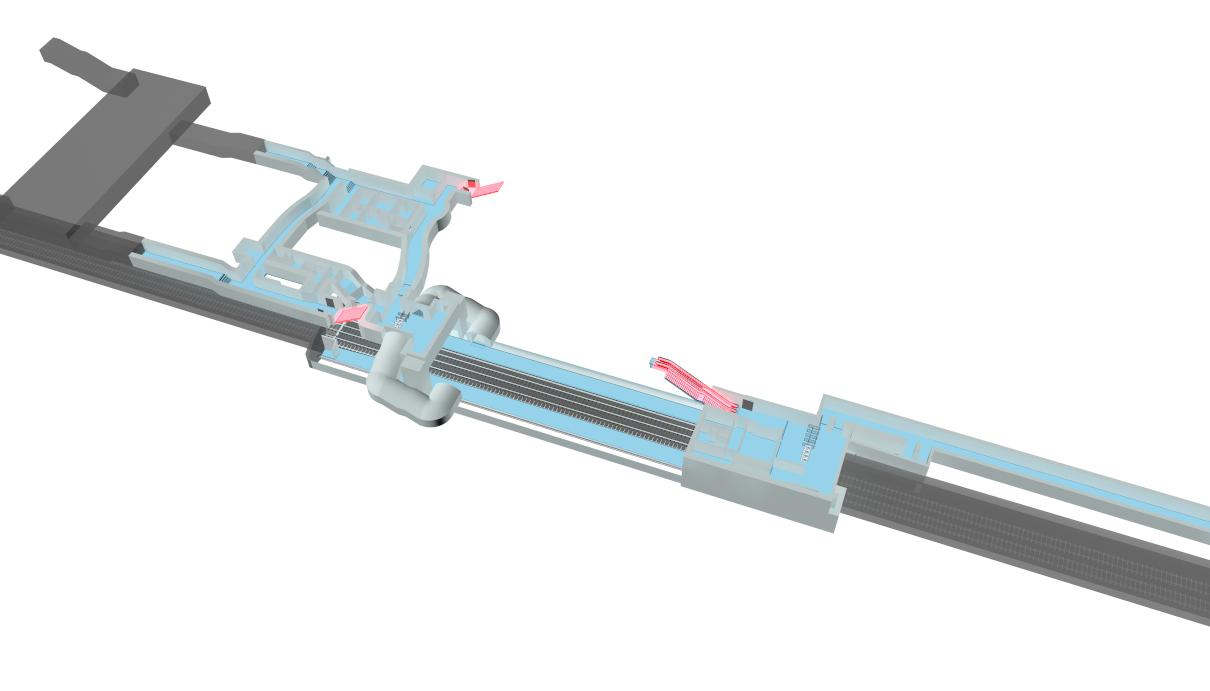
\includegraphics[width=\linewidth]{Figures/PdG-L3_schematic.jpg} 
  \caption{Schematic representation of PdG-L3. The accesses to platforms are highlighted in red. \cite{TMB}}
  \label{fig:PdG-L3_schematic}
\end{figure}

The public spaces are equipped with a Closed Circuit Television~(CCTV) for security reasons. The cameras of the CCTV-system provide images which contains the information how many people are on a dedicated time on a dedicated place. To gather these information the images are processed. In the following the CCTV system and the  images processing is described briefly.


\subsection{Passenger density data}
\label{subsec:PassengerDensityData}

Throughout the station a CCTV surveillance system is installed. 20~CCTV~cameras provides images mainly for security reasons.

We are using this system for the prediction of the number of passenger. There we gather from each camera how many people are visible.

Due to technical restriction a circuit design was implemented, meaning that the cameras provide subsequently the images. The circuit hold on each camera for 3  seconds. Consequently the in one minute one turn is conducted and the circuit starts with the first camera again.

Whenever camera pictures are processed the privacy issues are tackled. To ensure the privacy restrictions several actions took place.
First of all, all CCTV images needed for prediction purposes does not leave the station. To ensure this, the image processing is conducted on a dedicated computer especially bought for this purpose. The computer is located in a technical room within the station.
The images received on the computer are processed "on the fly" and thus not saved.
The first data which leaves the station are information five values: date, time, cameraID and number of passenger. These values are stored in the database.

 The images provided by each CCTV-camera are stored on a video recorder. A crowd density estimator processes the images and returns the number of passengers on this image. The number of passenger as well as date, time and the camera-ID are saved in a database.

For different reasons, e.g. bad camera picture, it is possible that the image processing fails. In this case the image processing return the error value "-1".
Figure~\ref{fig:CCTVimageProcessing} depict the processing chain.

\begin{figure}[htb]
  \centering
  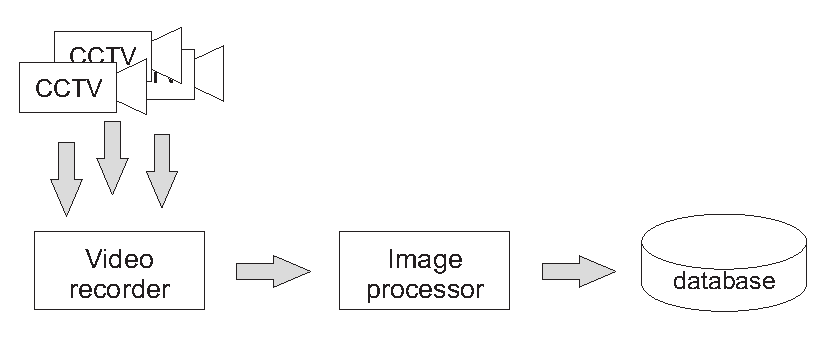
\includegraphics[width=\linewidth]{Figures/imageProcessing.pdf} 
  \caption{Gathering number of people out of the camera images.}
  \label{fig:CCTVimageProcessing}
\end{figure}

The CCTV and image processing runs 24~hours, 7~days a week. Each day 31680~datasets are saved to the database. Overall the database contains 90~days of data.
Figure~\ref{fig:rawData_week} illustrates exemplary the available values of a week. At a more detailed view of a day the service times are visible (Figure~\ref{fig:rawData_day}).

% one column
\begin{figure*}[tb]

  \centering

  \subfigure[Passenger density distribution of one camera during one week.] {
    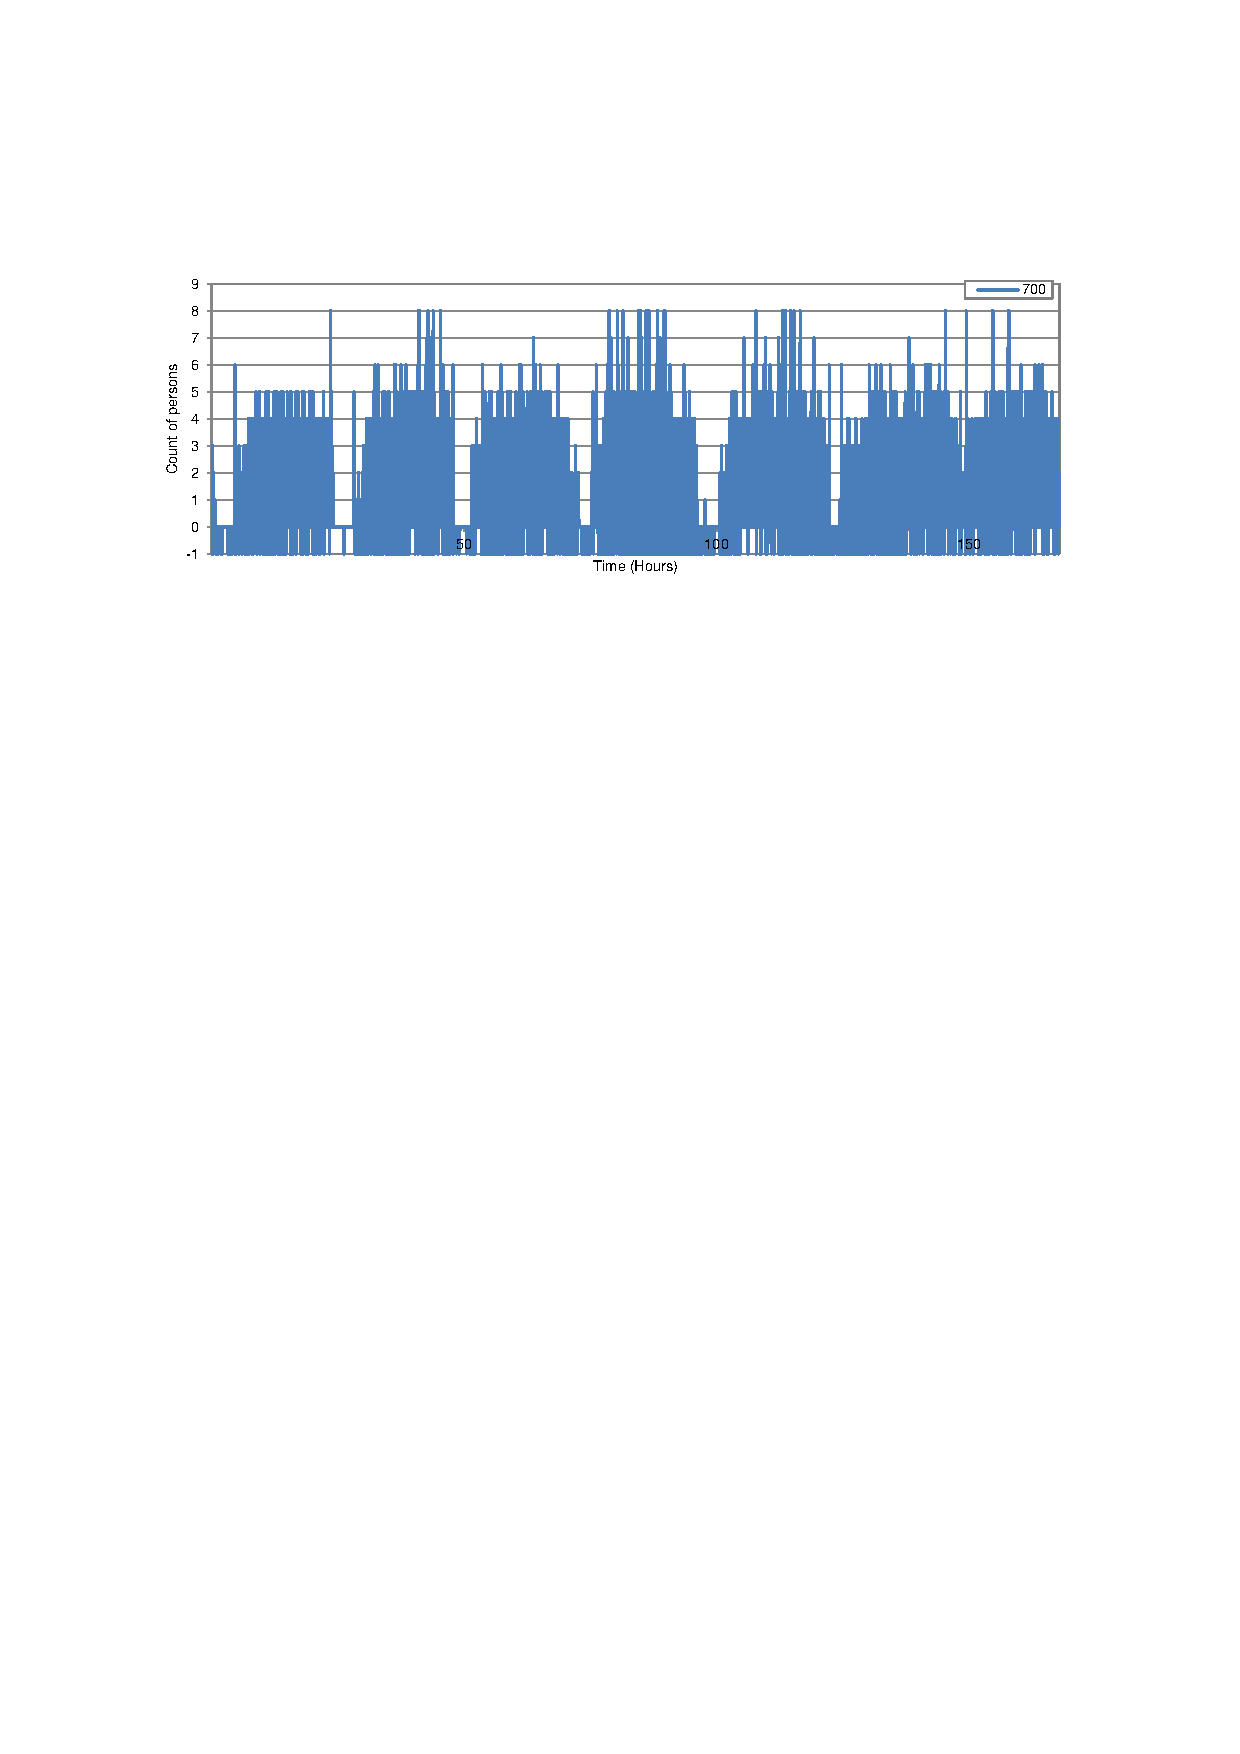
\includegraphics[width=0.46\textwidth]{Figures/rawData_week.pdf}
    \label{fig:rawData_week}
  }
  \hfill
  \subfigure[Passenger density distribution of one camera during one day.] {
    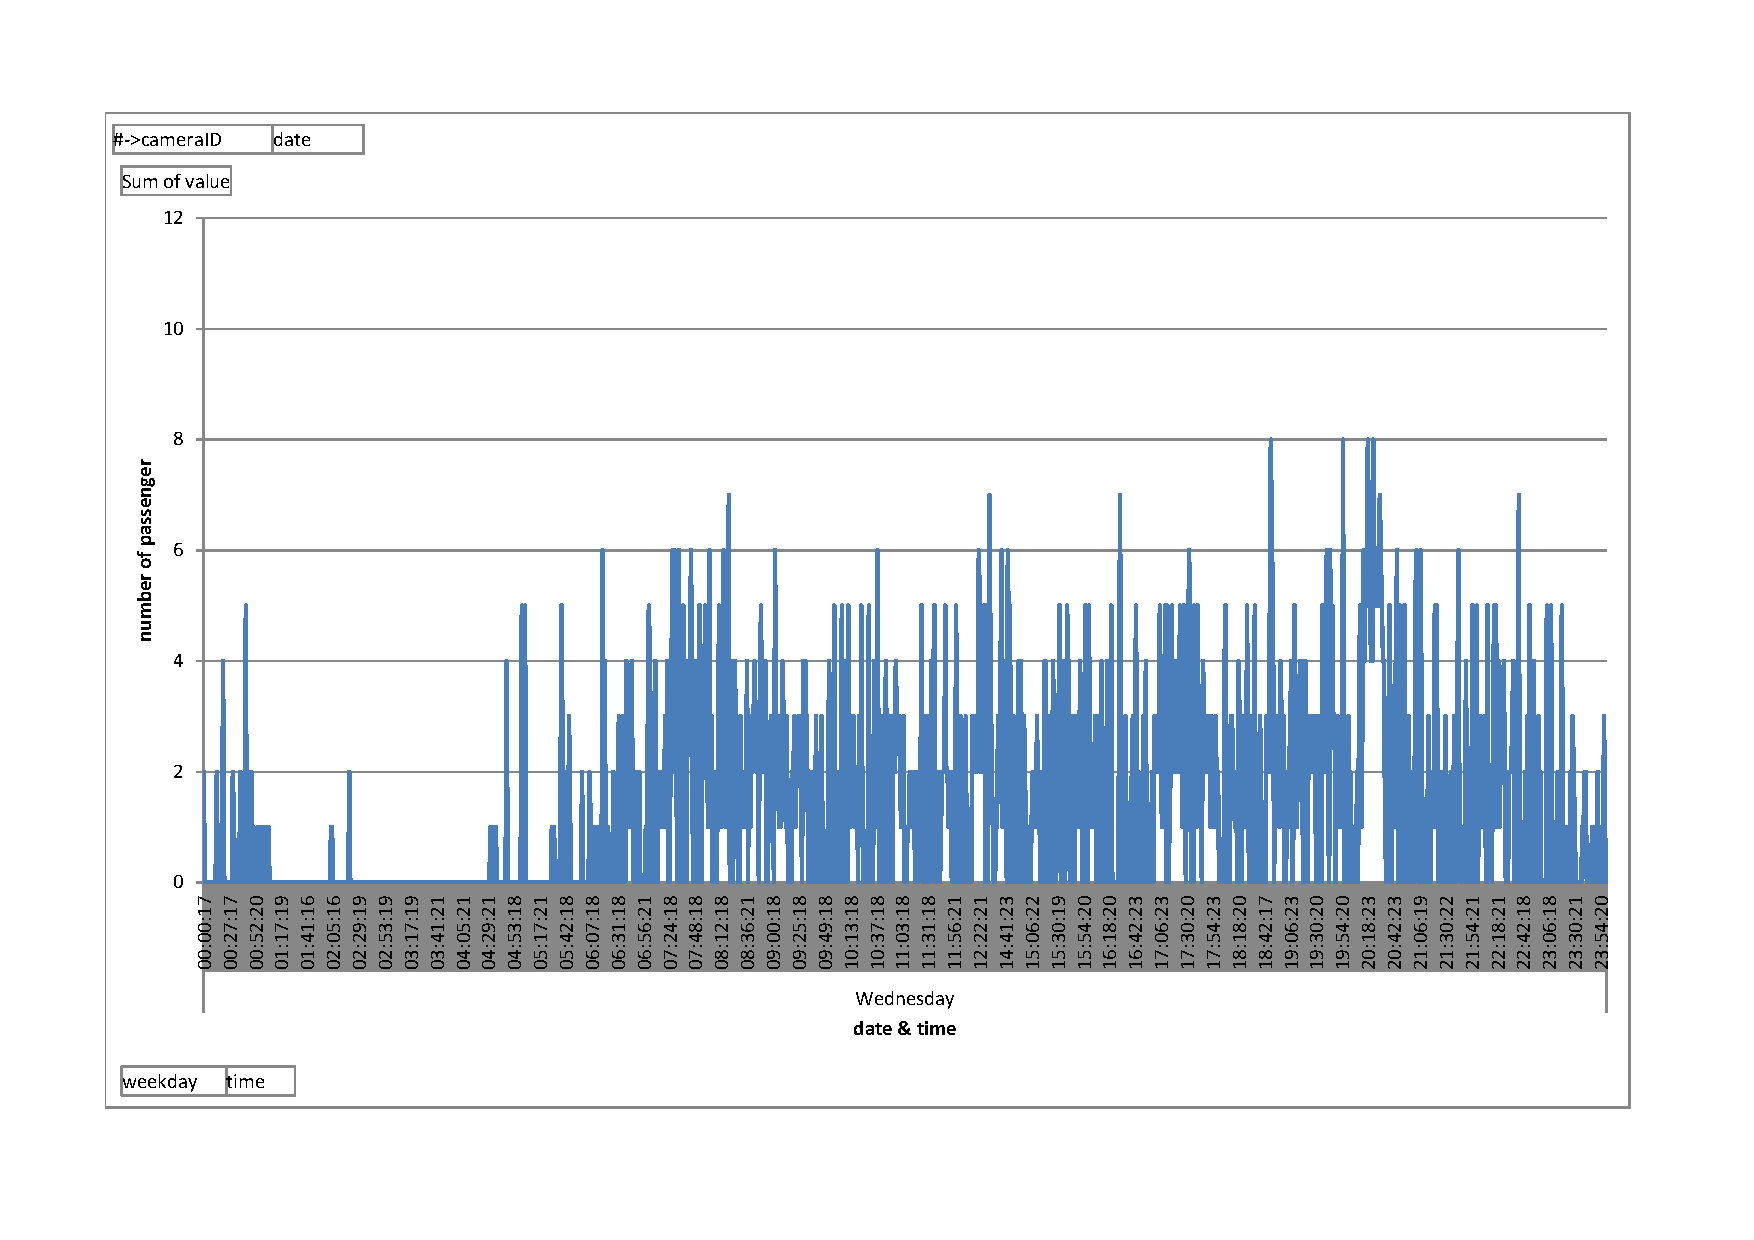
\includegraphics[width=0.46\textwidth]{Figures/rawData_day.pdf}
    \label{fig:rawData_day}
  }

  \caption{Passenger density distribution of one camera.~\cite{TMB}.}
  \label{fig:rawData}

\end{figure*}

